% !TeX encoding = UTF-8
% !TeX spellcheck = en_US
\section{Introduction}
In the last years, image classification processes like neural networks in the area of art-history and \emph{Heritage Informatics} have experienced a broad distribution \parencite{lang_AttestingSimilaritySupportingOrganizationStudy_2018}.
These methods face several challenges, including the handling of comparatively small amounts of data as well as high-dimensional data in the Digital Humanities. In most cases, these methods map the classification task to flat target space. This \enquote{flat} surface loses several relevant dimensions in the search for ontological uniqueness, including taxonomical, mereological, and associative relationships between classes, or the non-formal context, respectively.

The proposed solution by \citeauthor{donig_VomBildTextUndWieder_2019a} \parencite{donig_VomBildTextUndWieder_2019a} to expand the capabilities of visual classifiers is to take advantage of the greater expressiveness of text-based models. Here, a \emph{Convolutional Neural Network} (CNN) is used that output is not as usual a series of flat text labels but a series of semantically loaded vectors. These vectors result from a \emph{Distributional Semantic Model} (DSM) (\cite{lenci_DistributionalModelsWordMeaning_2018a}) which is generated from an in-domain text corpus.


Here, we propose an early implementation of this method and analyze the results.

The conducted experiment is based on the collation of two corpora: one text-based and a visual. From the text, a DSM is created and then queried for a list of target words that are functionally the labels that are manually given to the images. The result is a list of vectors that correspond to the target words leading to images that are annotated not only with a label but also with a unique vector. The images and vectors are used as training data for a CNN that, afterward, should be able to predict a vector for an unseen image. This prediction vector can be converted back to a word by the DSM using a nearest-neighbor algorithm. We are looking for richer representation in this process, so we choose the five nearest neighbors. The similarity measure is the cosine similarity for high-dimensional vector spaces between the given target vector and the prediction vector. We derive a positive classification result if the target label is within the list of five nearest neighbors of the prediction vector.

Moreover, we compare the results between the proposed classification method and a conventional classification method using the same CNN as for the vector-based experiment but a list of flat labels. Finally, we can show that the vector-based approach (judging from classification metrics) is equally performant or even better than the label-based version.


\section{Experiment Structure}
The experiment is based on one text and one visual corpus from the area of material culture research with a focus on neo-classical artifacts.

\subsection{Text Corpus}
The text corpus is compiled out of 44 sources that are available under a free and permissive license. It contains English specialist publications on furniture and spatial art, published from the end of the 19\textsuperscript{th} century to the middle of the 20\textsuperscript{th} century. In multiple steps, the corpus is cleaned and preprocessed. First, a series of standard NLP methods are applied like tokenization, sentence- and word splitting, normalization of numbers, and named entity recognition (NER). Since we used retro-digitized material from a different source, we implemented manual corrections for the most common errors (such as ligatures like \texttt{TT} that were misinterpreted as \texttt{U}). Another level of preprocessing consists of content-related augmentations. In particular, we normalized compound words and synonyms according to a specified list, which is based on an ontology, the \emph{Neoclassica-Ontology} \parencite{donig_NeoclassicaMultilingualDomainOntology_2016}. This resulted in the final text corpus of total \num{3067237} words comprised of \num{107518} basic word forms.

The DSM is created using the \emph{Indra Frameworks} \parencite{sales_IndraWordEmbeddingSemanticRelatedness_2018a} with a vector size of \num{50}, a word window size of \num{10}, and minimal word count of \num{5}. We used \emph{Skipgram} as the \emph{Word2Vec} model \parencite{mikolov_EfficientEstimationWordRepresentationsVector_2013} with negative sampling.

\subsection{Image Corpus}
The image corpus consists of \num{1231} images of neoclassical furniture in their entirety, which are permissive licensed\footnote{The corpus was compiled from collections from the Metropolitan Museum, New York, the Victoria \& Albert Museum, London, the Wallace Collection, London, and several contemporary pattern books.}. The images are either historical pictorial material or photographs from the modern as-built documentation. They are split into \num{28} different classes.

\subsection{Combined Corpus}
The nature of the experiment is \emph{proof-of-concept}, so we used a VGG-like architecture of a \enquote{simple} convolutional neural network\footnote{The CNN is built from three convolutional blocks with two consecutive Convolutional Layers each with 32/64/64 filters of size $ 3 \times 3 $. Each block is followed by a Maximum Pooling Layer with a size of $ 2 \times 2 $ and a Dropout Layer for regularization with a dropout rate of \num{0.25}. After the Convolutional Block, there are two Fully Connected Layers with \num{256} nodes and a Dropout Layer with a dropout rate of \num{0.5}. The weights and biases for the Convolutional and the Fully Connected Layers are initialized randomly. Their activation function is \emph{ReLU}. The last layer, the classification layer, is a Fully Connected Layer with \num{50} output nodes and a linear activation function. The optimization function of the chosen \emph{mean absolute error} function is \emph{RMSprop}. The implementation is done with Keras (\url{https://keras.io}) and TensorFlow (\url{https://tensorflow.org})}.

The independence and robustness of the train/test split are guaranteed with 5-fold cross-validation on \SI{80}{\percent} on the full corpus from which \SI{80}{\percent} are used for training and \SI{20}{\percent} for testing. The remaining \SI{20}{\percent} are treated as an evaluation set.

\begin{figure}
    \centering
    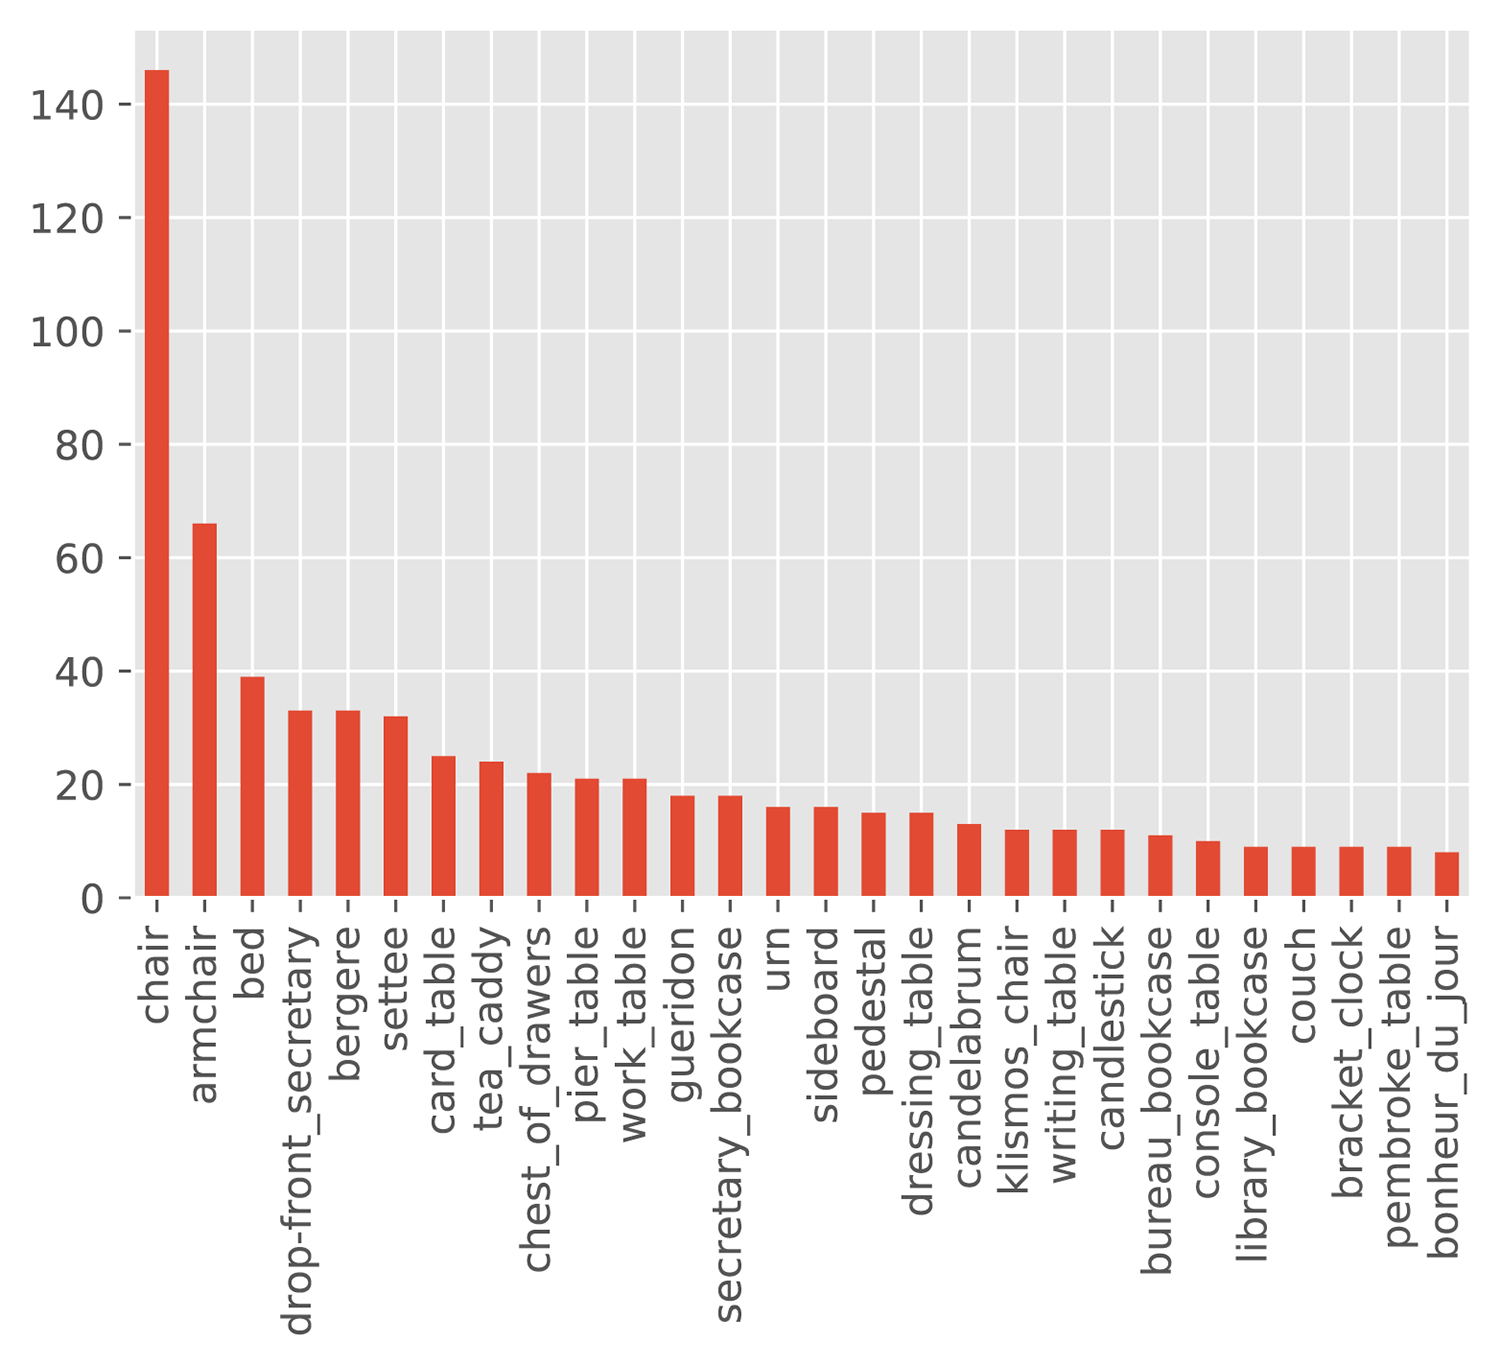
\includegraphics[height=.45\textheight]{class_distribution}
    \caption{Class distribution of the image corpus}
    \label{fig:class_distribution}
\end{figure}

The dataset is unbalanced, as can be seen in Fig.~\ref{fig:class_distribution}. During training, more prominent classes are weighted down and underrepresented classes are given a higher weight \parencite[p.~27]{johnson_SurveyDeepLearningClassImbalance_2019}. Apart from dropout during training for regularization, \emph{Early Stopping} was used to prevent overfitting.


\section{Results}

\subsection{Results for CNN trained on Word Vectors}

The Top-5 true-positive rate is \num{0.6052}, meaning that the gold label from the annotations is in \SI{60}{\percent} of the cases within the list of the five nearest neighbors.

However, the mathematical quality metric in itself represents only part of the overall picture. For this reason, a qualitative analysis of the results was performed.

A few true-positives show that, for example, the classification is by no means random but that the top 5 terms originate from the same semantic neighborhoods. They express several relationships of a taxonomical and associative nature.

As an example, the \emph{Roentgen} desk from the \emph{Victoria \& Albert} inventory in Fig.~\ref{fig:classification_same_object_1} is associated with the labels \texttt{dressing\_table}, \texttt{writing\_table} and \texttt{work\_table}. This triad is meaningful because many of these artifacts were multifunctional and fulfilled several of these functions. Besides, those artifacts that decidedly served only one purpose are constructively similar to the other types of furniture. The similarity of the three concepts thus emerges both on a semantic level (the distance of the words in the DSM, which in turn is the product of real-world distance) and on a visual level in the CNN (visual similarity of the form). Another image of the same object (see Fig.~\ref{fig:classification_same_object_2}) shows, on the other hand, that the method is consisted in itself---the top 4 nearest neighbors of the predicted vector are identical, although the photograph is taken from a different perspective---and, on the other hand, that the visual features within the CNN also affect the classification process. Since writing cabinets (\emph{secrétaires à abbatants}) are often displayed frontally, upright and with an open flap or drawer, their appearance in the image seems to have triggered a classification as a secretary. In the first image, however, the presence of drawers could have led to a classification as a chest-of-drawers, which is associated with drawers on a semantic level.

\begin{figure}
    \centering
    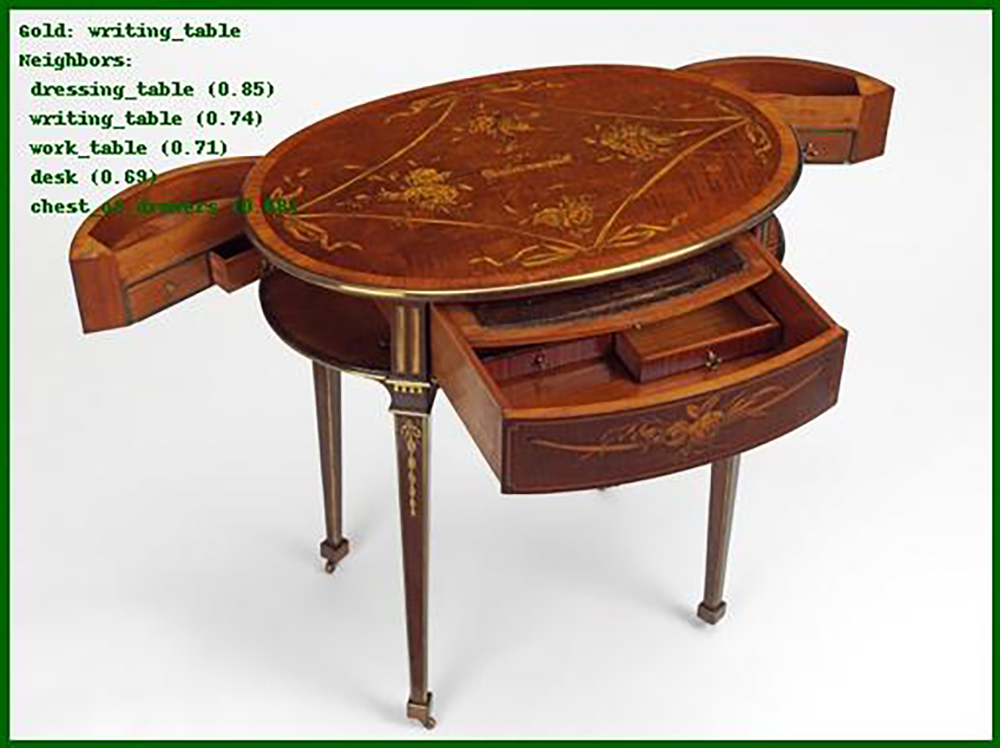
\includegraphics[height=.4\textheight]{classification_same_object_1}
    \caption{Differences in the classification of the same object (1)}
    \label{fig:classification_same_object_1}
\end{figure}

\begin{figure}
    \centering
    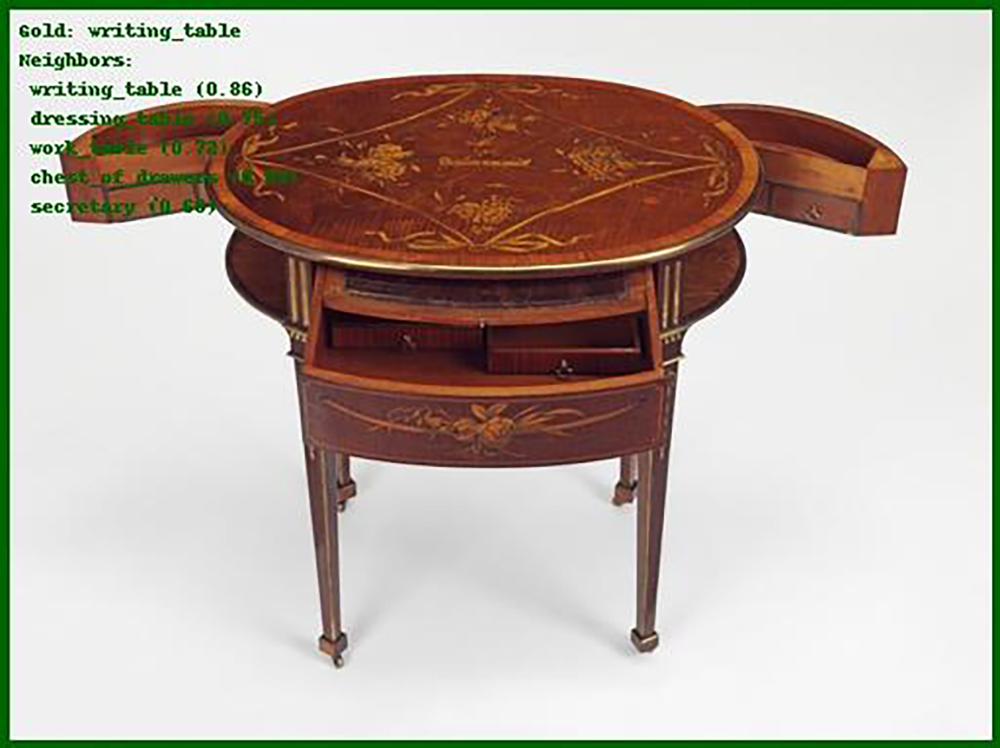
\includegraphics[height=.4\textheight]{classification_same_object_2}
    \caption{Differences in the classification of the same object (2)}
    \label{fig:classification_same_object_2}
\end{figure}


While the labels considered so far reflect the taxonomic relationships and all originate from the target words derived from the ontology, Fig.~\ref{fig:medici_vase} shows that the procedure can also generate labels for itself, purely data-driven. The crater vase shown was originally classified as an urn. The Top-2 words therefore also reflect taxonomic relationships (\enquote{urn}, \enquote{vase}). The other concepts reflect associative relationships. The label \texttt{bell} is a leftover from the data cleaning process of the text corpus to describe this kind of artifact. \enquote{Ovoid} refers to the egg stick decoration of the upper bead, which is often described with this adjective. This ornamentation seems at the same time to have an association with the rosette (patera). In this way, the target word \texttt{patera\_element} appears among the top-5 nearest neighbors, although only whole artifacts were annotated in the image corpus but not their decoration.


\begin{figure}
    \centering
    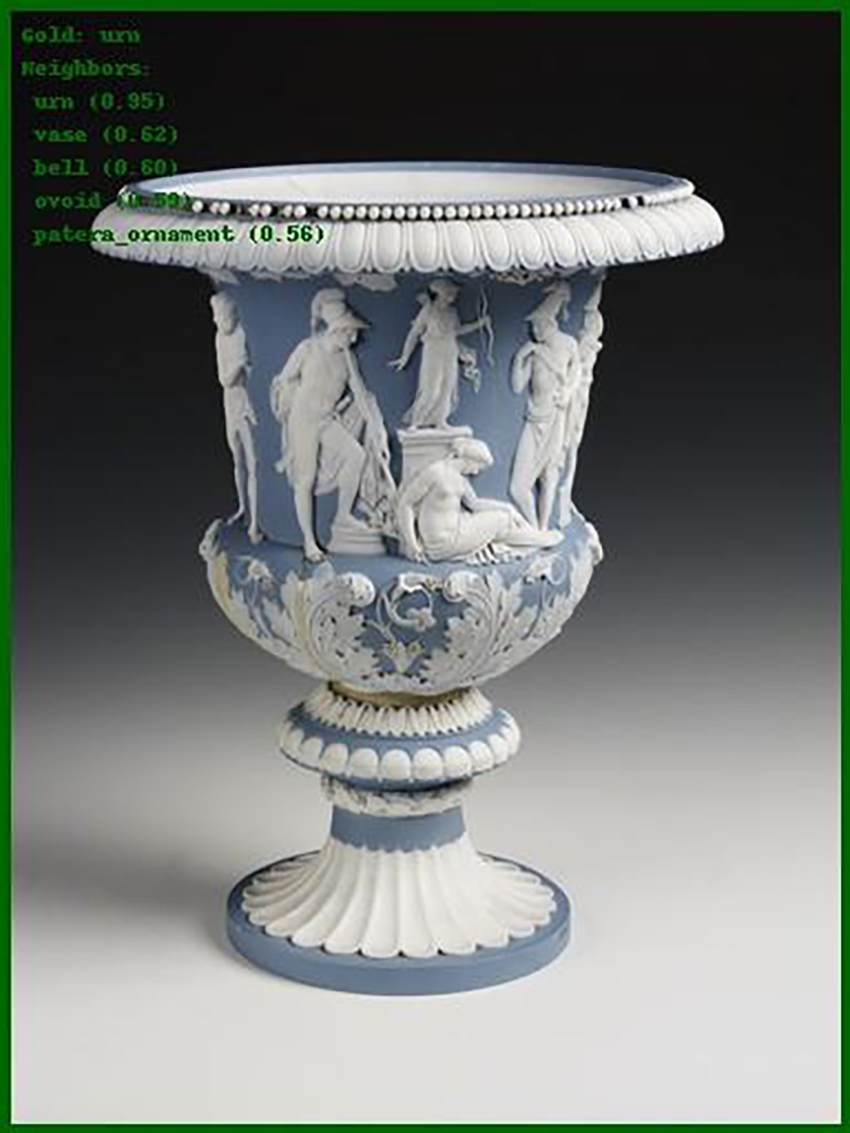
\includegraphics[height=.6\textheight]{medici_vase}
    \caption{A sèvres copy of a Medici vase results in a classification of associative labels.}
    \label{fig:medici_vase}
\end{figure}


An effect of the visual classifier cannot be excluded, as shown in Fig.~\ref{fig:misclassification}. The misclassification of the object, a small sewing table, led to consistent attributions in the area of seating and reclining furniture. Looking at the outer form of the artifact on a more abstract level, visual proximity to e.g. a (double)-camel-back sofa can be easily derived.


\begin{figure}
    \centering
    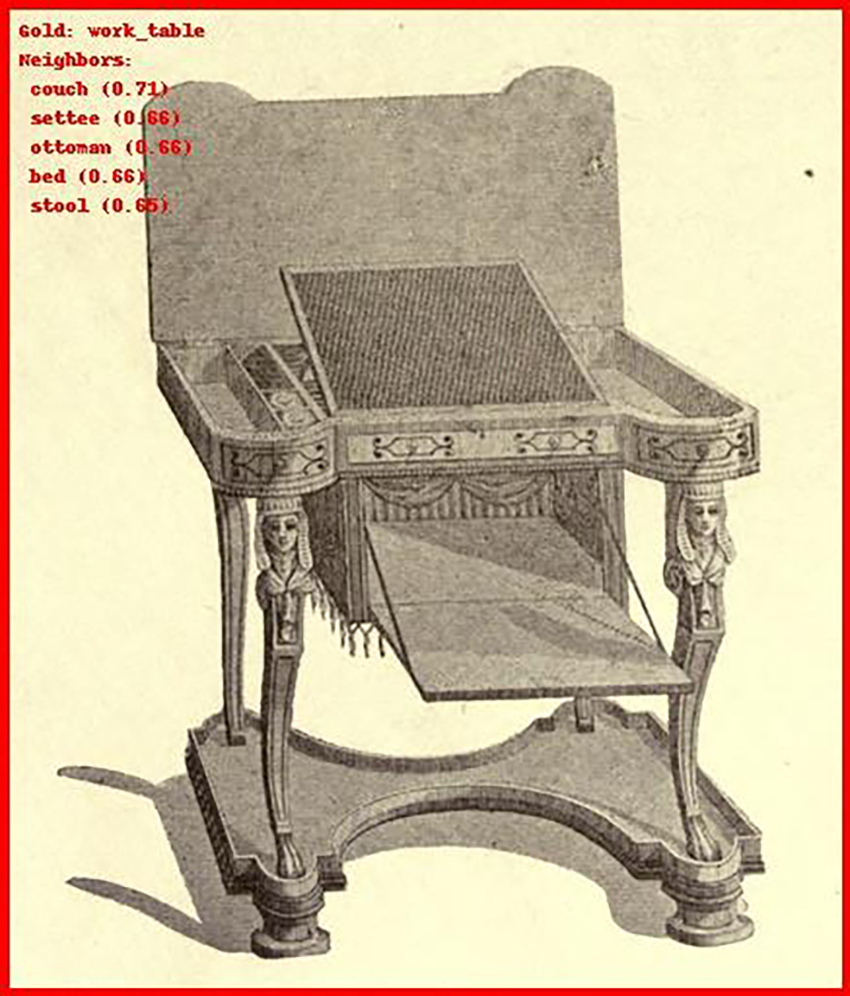
\includegraphics[height=.6\textheight]{misclassification}
    \caption{Misclassification of a sewing table in the proximity of seating furniture hierarchy.}
    \label{fig:misclassification}
\end{figure}


\subsection{Comparison to a CNN with flat labels}

To better estimate the differences between the two approaches (conventional classification by flat labels vs.~vector-based approach), we present a comparison between different metrics for both approaches.

\begin{table}
    \centering
    \begin{tabular}{lrr}
        \toprule
        Metric                     &   Vector-based &   Label-based \\ \midrule
        Top-1 Accuracy             &   \num{0.5378} &  \num{0.5302} \\
        Top-1 Precision            &   \num{0.3487} &  \num{0.4446} \\
        Top-1 Recall               &   \num{0.2974} &  \num{0.4044} \\
        Top-1 F1-Score             &   \num{0.2976} &  \num{0.3985} \\ \midrule
        Top-5 True-Positive-Rate   &   \num{0.6052} &  \num{0.8463} \\
        Top-5 False-Positive-Rate  &   \num{0.3948} &  \num{0.1537} \\
         \bottomrule
    \end{tabular}
    \caption{Results of different Metrics.}
    \label{tab:results}
\end{table}

As shown in Table~\ref{tab:results} the metrics are comparable.
% TODO: Why are the result worse than before?


Thus, the proposed approach not only improves the accuracy but also provides a richer description of the image.


\section{Conclusion and Outlook}
In this paper, we have presented a new multimodal approach for the classification of images based on the combination of NLP methods with image classification techniques. The goal was to classify objects not only according to a scheme of flat labels but in a more context-appropriate way, whereby the context informed by relevant domain-historical publications. This classification method offers access to the multidimensional embedding of artifacts in the real-world and their linguistic reflection. This circumstance is particularly useful for classifying multifunctional objects without having to resort to several classifiers and a complex annotation process with several labels. The results are encouraging. Even with a very simple  CNN, we achieve an accuracy of \num{0.54}.

As a next step, we want to train with a deeper CNN and an extended image corpus---to reduce known problems like overfitting. The comparative experiment with a conventional flat-label approach has shown that from an efficiency point-of-view, i.e., indirect metric comparison, our method not only provides comparable results but also provides a richer description of the image.


We will continue to work to better understand how a particular body of text is reflected int he labels that the DSM automatically assigns and that are not part of the list of target words. A better understanding of these processes seems particularly relevant given the relatively manageable text corpora that can be collated into specific topic complexes in the humanities. Last but not least, for this reason, we will consider the use of thesauri and dictionaries to create synonym lists for target words. Similarly, we are considering combining named entities into URIs. This would allow us to associate specific entities (e.g., workshops, ebenists, owners) with specific objects.

We think that multimodal access provides particularly efficient access to humanities and cultural studies corpora that are small and domain-restricted compared to corpora of other disciplines in the natural and social sciences.
